\documentclass[9pt,twocolumn,twoside]{pnas-new}
% Use the lineno option to display guide line numbers if required.
% Note that the use of elements such as single-column equations
% may affect the guide line number alignment. 

\templatetype{pnasresearcharticle} % Choose template 
% {pnasresearcharticle} = Template for a two-column research article
% {pnasmathematics} = Template for a one-column mathematics article
% {pnasinvited} = Template for a PNAS invited submission

\title{A Serverless Tool for Platform Agnostic Computational Experiment Management}

% Use letters for affiliations, numbers to show equal authorship (if applicable) and to indicate the corresponding author
\author[a,b,$\dagger$]{Gregory Kiar}
\author[a]{Shawn T. Brown} 
\author[*,c]{Tristan Glatard} 
\author[*,a,b,d]{Alan C. Evans}

\affil[a]{Montreal Neurological Institute, McGill University, Montreal, Canada}
\affil[b]{Department of Biomedical Engineering, McGill University, Montreal, Canada}
\affil[c]{Department of Computer Science, Concordia University, Montreal, Canada}
\affil[d]{Department of Neurology and Neurosurgery, McGill University, Montreal, Canada}
\affil[*]{Co-senior author}
\affil[$\dagger$]{Corresponding author: greg.kiar\@mcgill.ca}

% Please give the surname of the lead author for the running footer
\leadauthor{Kiar} 

% Please add here a significance statement to explain the relevance of your work
\significancestatement{Authors must submit a 120-word maximum statement about the significance of their research paper written at a level understandable to an undergraduate educated scientist outside their field of speciality. The primary goal of the Significance Statement is to explain the relevance of the work in broad context to a broad readership. The Significance Statement appears in the paper itself and is required for all research papers.}

% Please include corresponding author, author contribution and author declaration information
\authorcontributions{GK did things, SB provided help and advice, TG provided help and advice and co-supervised, AE co-supervised.}
\authordeclaration{The authors declare no conflicts of interest in this work.}
% \equalauthors{\textsuperscript{1}A.O.(Author One) and A.T. (Author Two) contributed equally to this work (remove if not applicable).}
% \correspondingauthor{\textsuperscript{2}To whom correspondence should be addressed. E-mail: greg.kiar\@mcgill.ca}

% Keywords are not mandatory, but authors are strongly encouraged to provide them. If provided, please include two to five keywords, separated by the pipe symbol, e.g:
\keywords{Keyword 1 $|$ Keyword 2 $|$ Keyword 3 $|$ ...} 

\begin{abstract}
Please provide an abstract of no more than 250 words in a single paragraph. Abstracts should explain to the general reader the major contributions of the article. References in the abstract must be cited in full within the abstract itself and cited in the text.
\end{abstract}

\dates{This manuscript was compiled on \today}
% \doi{\url{www.pnas.org/cgi/doi/10.1073/pnas.XXXXXXXXXX}}

\begin{document}

% Optional adjustment to line up main text (after abstract) of first page with line numbers, when using both lineno and twocolumn options.
% You should only change this length when you've finalised the article contents.
\verticaladjustment{-2pt}

\maketitle
\thispagestyle{firststyle}
\ifthenelse{\boolean{shortarticle}}{\ifthenelse{\boolean{singlecolumn}}{\abscontentformatted}{\abscontent}}{}

% If your first paragraph (i.e. with the \dropcap) contains a list environment (quote, quotation, theorem, definition, enumerate, itemize...), the line after the list may have some extra indentation. If this is the case, add \parshape=0 to the end of the list environment.
%\dropcap{T}his PNAS journal template is provided to help you write your work in the correct journal format.  Instructions for use are provided below.

\begin{itemize}
\item Computational sciences are becoming more and more common and necessary.
\item Standards are emerging to aid in the reproducibility and shareability of tools and data
\begin{itemize}
\item Boutiques
\item BIDS
\item BIDS apps
\end{itemize}
\item Virtualization tools make analysis software increasingly portable
\begin{itemize}
\item Docker
\item Singularity
\end{itemize}
\item Platforms enable running workflows at scale on a variety of computational resources
\begin{itemize}
\item CBRAIN
\item LONI
\item Nipype
\end{itemize}
\item Execution provenance is becoming increasingly focal and we are recognizing its importance
\begin{itemize}
\item NIDM (neuroscience prov)
\item ReCAP (infrastructure stats/prov)
\item Reprozip (file i/o prov)
\end{itemize}
\item Tools have varying use-cases and barriers for adoption
\begin{itemize}
\item CBRAIN/LONI are designed for production-level pipelines
\item Nipype is complex for tool consumption or simple workflow construction
\item NIDM is very rich and requires deep integration with the tool
\item ReCAP monitors machine resources in virtual machine-based clouds
\item Reprozip has limited compatibility when run around containers, depending on infrastructure
\end{itemize}
\item Clowdr accessibly leverages these approaches where possible and builds-up pipelines with increased deployability, provenance, and shareability
\begin{itemize}
\item Accessible deployment environment closer to development
\item Makes tool consumption very easy
\item Records rich cpu and memory provenance everywhere
\item Records reprozip provenance whenever possible
\item Enables apps/containers that leverage NIDM, Nipype, Reprozip, etc., internally to do their thing, and only adds further richness to provenance records
\item Provides accessible web interface to browse, download, and share executions
\end{itemize}
\end{itemize}

\section*{Methods}
\begin{itemize}
\item Data awareness with BIDS
\item Cluster and cloud interface with SLURM and Amazon APIs (and extensible)
\item Containerization with Singularity or Docker
\item Parameter sweeping with boutiques/clowdr
\item Tool encapsulation with Boutiques
\item Provenance capture using reprozip*, memprofile, cpu-timing
\item Data sharing and publication with Flask
\item Figure 1: workflow diagrams (done)
\item Supplement repos?
\begin{itemize}
\item Dockerfile
\item Boutiques descriptor
\item Invocations
\item Clowdr command
\item Dataset
\end{itemize}
\end{itemize}

\subsection*{Results}
\begin{itemize}
\item Figure 2: instructions infographic (i.e. steps to use clowdr)
\item Figure 3: we ran, find provenance “here” (i.e. clowdr share)
\begin{itemize}
\item running ndmg on hcp data (compute canada)
\item 1-voxel analysis (compute canada cloud?)
\item Bids example (amazon)
\end{itemize}
\item example provenance analysis (i.e. instance size optimization)
\begin{itemize}
\item Mem usage comparisons (do)
\item CPU usage comparisons (do)
\end{itemize}
\end{itemize}

\subsection*{Discussion}
\begin{itemize}
\item other uses of provenance information
\begin{itemize}
\item Reprozip trace comparisons (cite)
\item Extrapolate for informed decision making on cloud resource selection (cite)
\end{itemize}
\end{itemize}


\subsection*{Format}

Many authors find it useful to organize their manuscripts with the following order of sections;  Title, Author Affiliation, Keywords, Abstract, Significance Statement, Results, Discussion, Materials and methods, Acknowledgments, and References. Other orders and headings are permitted.

\subsection*{References}

References should be cited in numerical order as they appear in text; this will be done automatically via bibtex, e.g. \cite{belkin2002using} and \cite{berard1994embedding,coifman2005geometric}. All references should be included in the main manuscript file.  

\subsection*{Data Archival}

PNAS must be able to archive the data essential to a published article. Where such archiving is not possible, deposition of data in public databases, such as GenBank, ArrayExpress, Protein Data Bank, Unidata, and others outlined in the Information for Authors, is acceptable.


% \begin{figure}%[tbhp]
%   \centering
%   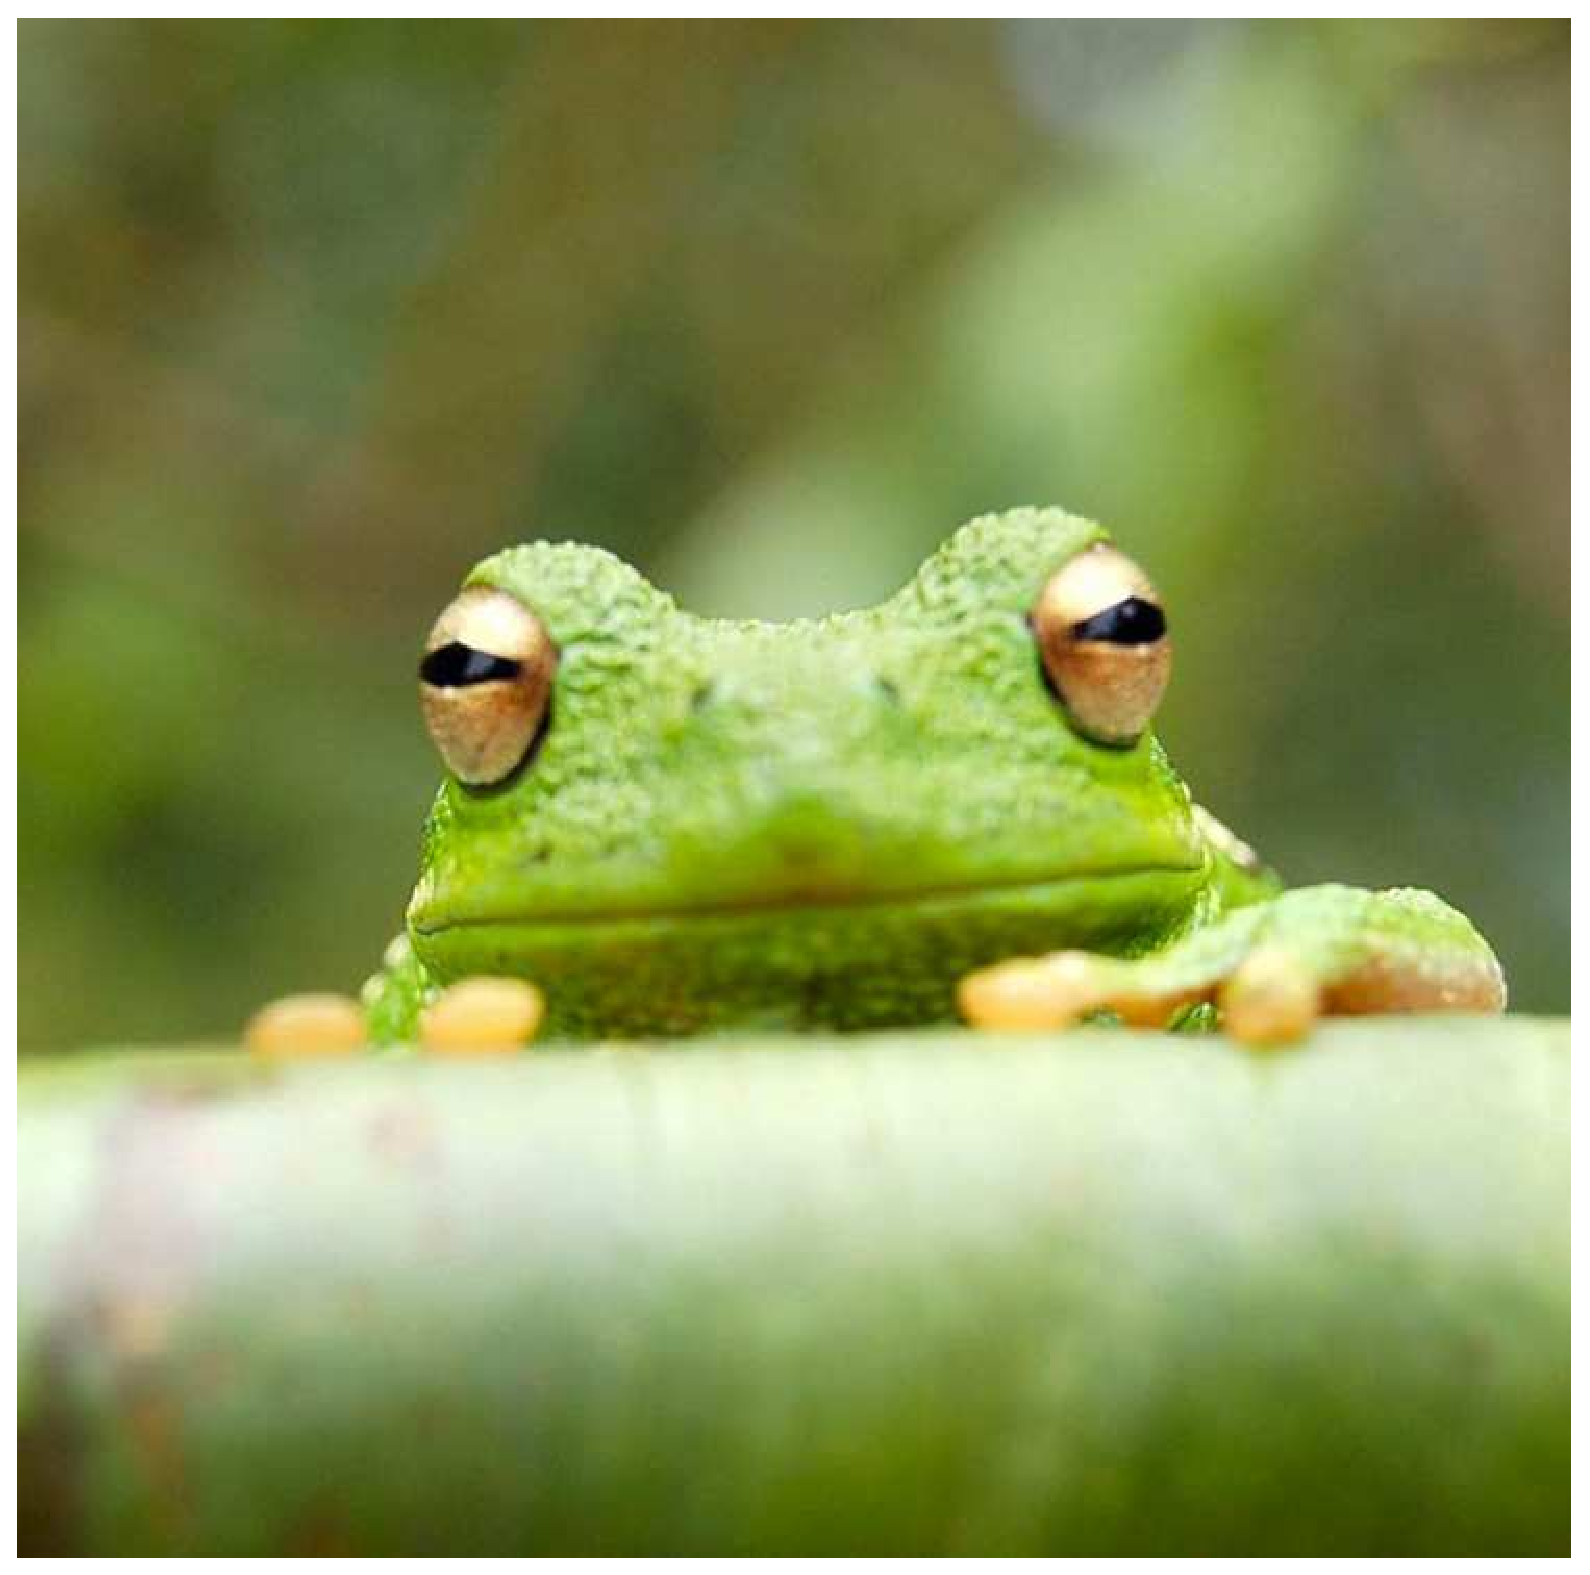
\includegraphics[width=.8\linewidth]{frog}
%   \caption{Placeholder image of a frog with a long example caption to show justification setting.}
%   \label{fig:frog}
% \end{figure}


% \begin{SCfigure*}[\sidecaptionrelwidth][t]
%   \centering
%   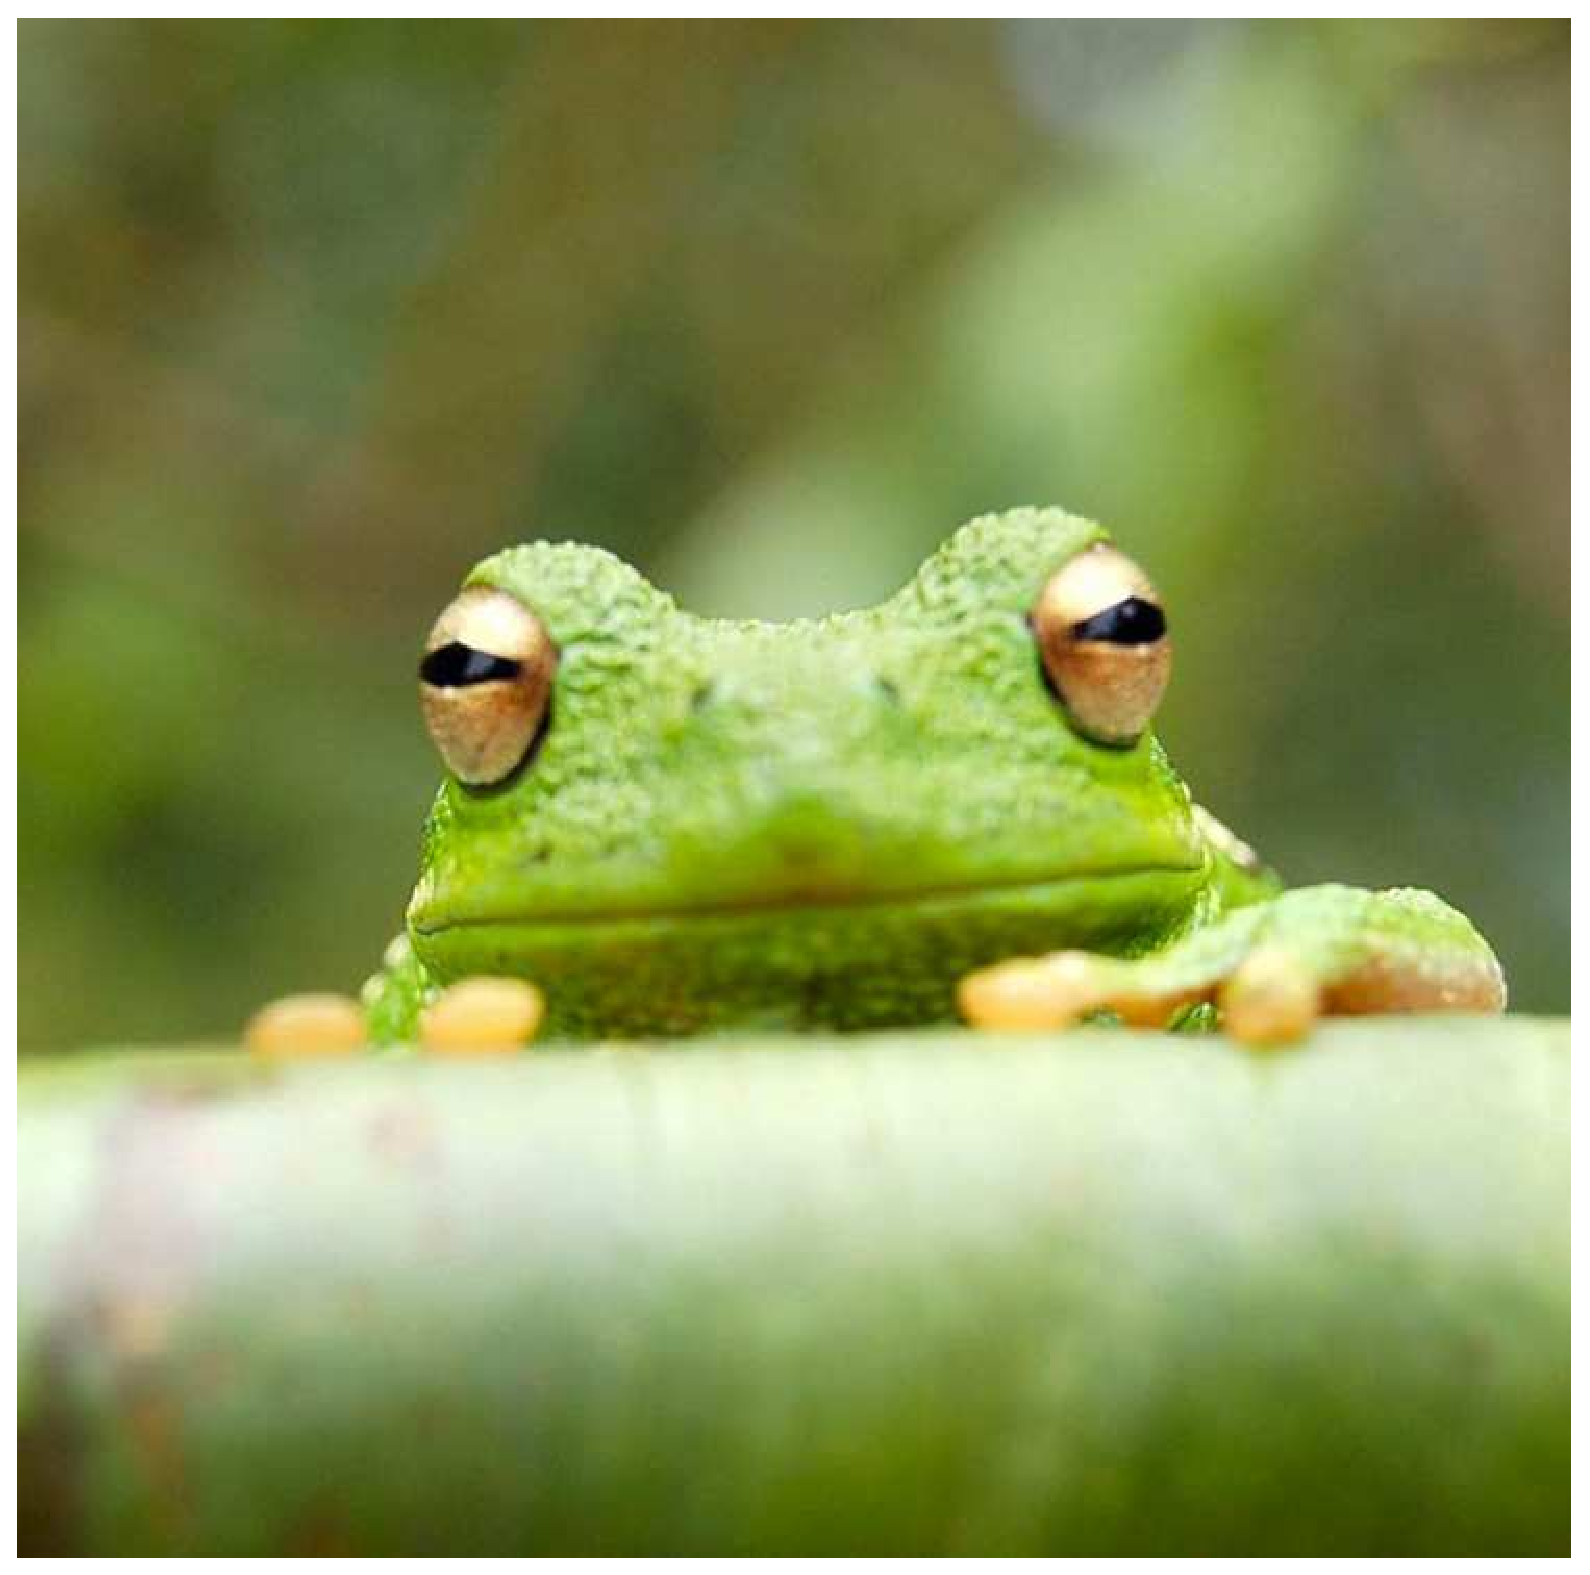
\includegraphics[width=11.4cm,height=11.4cm]{frog}
%   \caption{This caption would be placed at the side of the figure, rather than below it.}\label{fig:side}
% \end{SCfigure*}

\subsection*{Digital Figures}
\label{sec:figures}

Figure \ref{fig:frog} shows an example of how to insert a column-wide figure. To insert a figure wider than one column, please use the \verb|\begin{figure*}...\end{figure*}| environment. Figures wider than one column should be sized to 11.4 cm or 17.8 cm wide. Use \verb|\begin{SCfigure*}...\end{SCfigure*}| for a wide figure with side captions.

\subsection*{Single column equations}

Authors may use 1- or 2-column equations in their article, according to their preference.

To allow an equation to span both columns, options are to use the \verb|\begin{figure*}...\end{figure*}| environment mentioned above for figures, or to use the \verb|\begin{widetext}...\end{widetext}| environment as shown in equation \ref{eqn:example} below.

Please note that this option may run into problems with floats and footnotes, as mentioned in the \href{http://texdoc.net/pkg/cuted}{cuted package documentation}. In the case of problems with footnotes, it may be possible to correct the situation using commands \verb|\footnotemark| and \verb|\footnotetext|.

%% Do not use widetext if paper is in single column.
% \begin{widetext}
%   \begin{align*}
%     (x+y)^3&=(x+y)(x+y)^2\\
%            &=(x+y)(x^2+2xy+y^2) \numberthis \label{eqn:example} \\
%            &=x^3+3x^2y+3xy^3+x^3. 
%   \end{align*}
% \end{widetext}

% \begin{table}%[tbhp]
%   \centering
%   \caption{Comparison of the fitted potential energy surfaces and ab initio benchmark electronic energy calculations}
%   \begin{tabular}{lrrr}
%     Species & CBS & CV & G3 \\
%     \midrule
%     1. Acetaldehyde & 0.0 & 0.0 & 0.0 \\
%     2. Vinyl alcohol & 9.1 & 9.6 & 13.5 \\
%     3. Hydroxyethylidene & 50.8 & 51.2 & 54.0\\
%     \bottomrule
%   \end{tabular}
%   \addtabletext{nomenclature for the TSs refers to the numbered species in the table.}
% \end{table}

\subsection*{Supporting Information (SI)}

The main text of the paper must stand on its own without the SI. Refer to SI in the manuscript at an appropriate point in the text. Number supporting figures and tables starting with S1, S2, etc. Authors are limited to no more than 10 SI files, not including movie files. Authors who place detailed materials and methods in SI must provide sufficient detail in the main text methods to enable a reader to follow the logic of the procedures and results and also must reference the online methods. If a paper is fundamentally a study of a new method or technique, then the methods must be described completely in the main text. Because PNAS edits SI and composes it into a single PDF, authors must provide the following file formats only.

\subsubsection*{Appendices}

PNAS prefers that authors submit individual source files to ensure readability. If this is not possible, supply a single PDF file that contains all of the SI associated with the paper. This file type will be published in raw format and will not be edited or composed.

\acknow{Please include your acknowledgments here, set in a single paragraph. Please do not include any acknowledgments in the Supporting Information, or anywhere else in the manuscript.}
\showacknow{} % Display the acknowledgments section

% \pnasbreak splits and balances the columns before the references.
% Uncomment \pnasbreak to view the references in the PNAS-style
% If you see unexpected formatting errors, try commenting out \pnasbreak
% as it can run into problems with floats and footnotes on the final page.
%\pnasbreak

% Bibliography
\section*{References}
\bibliography{pnas-sample}

\end{document}
